% If I add all results to the Evaluation chapter, there's no need for a Results chapter.

% This will depend on how I structure the document once I start writing the experiments and results sections. For now, this stays empty.

\chapter{Results and Discussion}
In this chapter, the results from the experiment will be discussed.

\section{Results}
This section will introduce the results from the experiments.

\subsection{Masking Ratio for Masked Language Modeling}
The results from masking ratio for \acrshort{mlm} is shown on Table \ref{tb:fixed_mlm}. From Table \ref{tb:fixed_mlm} the metric measures the percentage of times the correct image is among the top K retrieved images for a given text query. Common values for K include 1, 5, and 10, represented as R@1, R@5, and R@10 respectively. The highest results for each metrics are shown bold.
The results from Table \ref{tb:fixed_mlm} shows that prediction accuracy differs below 2\%. For R@1 masking ratio of 30\% had the highest accuracy, but 15\% marked the highest for r@5 and r@10. There was 0.3\% to 0.55\% difference was observed from the results in Table \ref{tb:fixed_mlm}, and no change in performance was observed by changing the mask rate.
Table \ref{tb:time_variant_mlm} shows that the masking ratio did not affect drastically to the prediction. 
%For the time variant masking ratio also did not change the results at all. 

\cite{Bai2023RaSaRA} used 15\% of masking ratio for their methods, but even though the accuracy did not get better.

\begin{table}[htbp]
    \centering
    \caption{Result for masking fixed masking ratio in \acrshort{mlm}}
    \label{tb:fixed_mlm}
    
    \begin{tabular}{rcccc}
      masking ratio & r@1 & r@5 & r@10 & mAP\\ \hline
      15\% & 76.51 & \textbf{90.20} & \textbf{94.25} & 69.38 \\
      20\% & 76.64 & 89.90 & 93.70 & 70.27 \\
      25\% & 76.23 & 89.86 & 93.79 & 70.22 \\
      30\% & \textbf{76.72} & 89.77 & 93.60 & \textbf{70.30} \\
      35\% & 76.61 & 89.77 & 93.47 & 70.26 \\
      40\% & 76.56 & 89.88 & 93.47 & 70.26
    \end{tabular}
\end{table}

\begin{table}[htbp]
  \centering
  \caption{Result for time variant masking ratio in \acrshort{mlm}}
  \label{tb:time_variant_mlm}
  \begin{tabular}{rcccc}
    \centering
    masking ratio & r@1 & r@5 & r@10 & mAP\\ \hline
    linear increase & 76.62 & 89.88 & 93.62 & \textbf{70.36} \\
    linear decrease & \textbf{76.70} & 89.85 & 93.58 & 70.21 \\
    cosine increase & 76.54 & 90.04 & \textbf{94.02} & 70.15 \\
    cosine decrease & 76.21 & \textbf{90.09} & 93.65 & 70.21 \\
  \end{tabular}
\end{table}


\subsection{Masking Ratio for Momentum-based Replaced Token Detection}
% The results for \acrshort{mrtd} is shown in table \ref{tb:mrtd_fixed} for fixed masking ratio and table \ref{tb:mrtd_time_variant} for time variant masking ratio. From table \ref{tb:mrtd_fixed} 

% The performance from table \ref{tb:fixed_mlm} shows that r@1 had the best performance at a 40\% masking ratio with a value of 75.80. For r@5, 30\% masking ratio reached the highest value of 93.92\%. R@10 did not make any better progress from r@5 which scored 93.97\%. From mAP the 30\% masking ratio scored the highest, but the difference was lower than 1\%.  This suggests that the model's performance can vary slightly depending on the specific evaluation metric prioritized. 

% The model performance was also consistent across time variant masking ratio from table \ref{tb:mrtd_time_variant}. R@1 had better performance compared with fixed masking ratio, but overall, not much of a improvements was observed. 

The results for \acrshort{mrtd} are shown in Table \ref{tb:fixed_mlm} for fixed masking ratio and Table \ref{tb:mrtd_time_variant} for time variant masking ratio.

From Table \ref{tb:mrtd_fixed}, the performance indicates that r@1 achieved the best performance at a 40\% masking ratio with a value of 75.80. For r@5, the highest value of 93.9 was reached at a 30\% masking ratio. r@10 reached a peak value of 93.97 at a 40\% masking ratio, only marginally higher than the value at 30\%. In terms of mAP, the 30\% masking ratio scored the highest at 68.81, though the differences among masking ratios were relatively small, less than 1\%. This suggests that the model's performance can vary slightly depending on the specific evaluation metric prioritized.

The model's performance was also consistent across the time variant masking ratios shown in Table \ref{tb:time_variant_mlm}. r@1 had a better performance compared with the fixed masking ratio, with the highest value being 76.46 for linear decrease. However, overall improvements were minimal.

% \begin{figure}
%     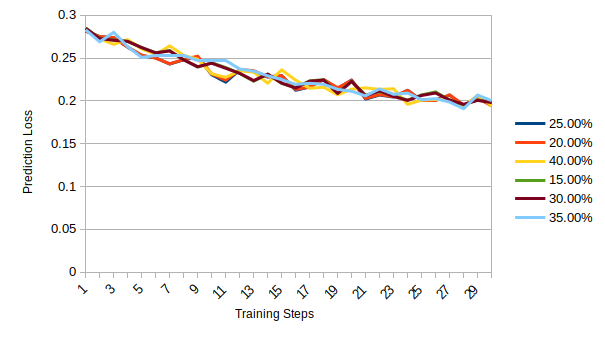
\includegraphics[width=\linewidth]{img/mrtd_prd_loss.png}
%     \caption{Prediction loss in training steps}
%     \label{img:mrtd_prd_loss}
% \end{figure}

% \begin{figure}
%     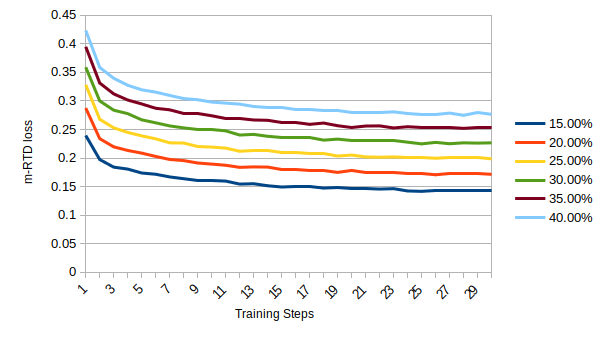
\includegraphics[width=\linewidth]{img/mrtd_loss.png}
%     \caption{MRTD Loss in training steps}
%     \label{img:mrtd_loss}
% \end{figure}

\begin{table}[htbp]
  \centering
  \caption{Result for fixed masking ratio on m-RTD}
  \label{tb:mrtd_fixed}
  \begin{tabular}{rcccc}
    masking ratio & r@1 & r@5 & r@10 & mAP \\ \hline
    15\% & 75.42 & 90.20 & 93.83 & 68.56 \\
    20\% & 75.58 & 90.35 & 93.91 & 68.73 \\
    25\% & 75.63 & 90.09 & 93.83 & 68.76 \\
    30\% & 75.57 & \textbf{90.37} & 93.92 & \textbf{68.81} \\
    35\% & 75.03 & 90.14 & 93.89 & 68.57 \\
    40\% & \textbf{75.80} & 90.27 & \textbf{93.97} & 68.73
  \end{tabular}
\end{table}

\begin{table}[htbp]
  \centering
  \caption{Result for time variant masking ratio from 2\% to 40\%}
  \label{tb:mrtd_time_variant}
  \begin{tabular}{rcccc}
    \centering
    masking ratio & r@1 & r@5 & r@10 & mAP\\ \hline
    linear increase & 76.20 & 90.11 & 93.94 & 70.22 \\
    linear decrease & \textbf{76.46} & 89.78 & 93.62 & \textbf{70.34} \\
    cosine increase & 75.91 & 89.85 & 93.89 & 68.40 \\
    cosine decrease & 75.99 & \textbf{90.25} & \textbf{94.01} & 68.73 \\
  \end{tabular}
\end{table}


\section{Discussion}
\subsection{Impact of Masking Ratio}

The experiments demonstrate that the effect of changing the masking ratio trivial towards the performance of \acrshort{rasa}. \cite{yang2023learningbettermaskingbetter} demonstrated in their work that in pre-training, when the masking ratio is decreasing, the model adaptively focus on different aspects of the data, potentially enhancing its ability to learn robust representations. This adaptive approach improved the model's capacity to handle the complexities inherent in \acrshort{vlm}. However, the results from our experiment tells that changing the masking ratio on fine-tuning did not make an improvements. 

Tables \ref{tb:fixed_mlm} and \ref{tb:time_variant_mlm} summarize the results for fixed and time-variant masking ratios in \acrshort{mlm}, respectively. Notably, the model showed only minimal variations in performance across different masking ratios. For instance, a 30\% fixed masking ratio achieved the highest R@1 score of 76.72, while a 15\% ratio performed best for R@5 and R@10, achieving scores of 90.20 and 94.25, respectively. The differences in mAP were marginal, indicating that the choice of masking ratio has a limited impact on the model's overall performance.

In terms of time-variant masking ratios, the linear increase strategy resulted in the highest mAP of 70.36, although the variations were again minimal. This suggests that while different masking strategies can affect specific performance metrics slightly, the overall impact remains limited.

Fig \ref{fig:mlm_1} and \ref{fig:mlm_6} provided crucial insights into how the model's attention changes with different masking ratios. The \acrshort{gradcam} method generates localization maps that highlight the regions of an image most relevant to the model's predictions. By analyzing these maps, it was observed that the areas of focus shifted slightly with changes in masking ratios.

{\color{red} explain further}
For example, at a lower masking ratio (Fig \ref{fig:mlm_1}), the model tended to focus on more specific details within the image, whereas higher masking ratios (Fig \ref{fig:mlm_6}) led to broader attention spans across larger regions. For visual grounding for word `man', the lower masking ratio focuses specifically to the mans face, whereas the high masking ratio attention broadens to cover larger regions of the image. Since recognition accuracy does not change with different mask rates, it can be inferred that the model is able to maintain an overall understanding of the image, even if certain details are obscured.  


\begin{figure}[htbp]
  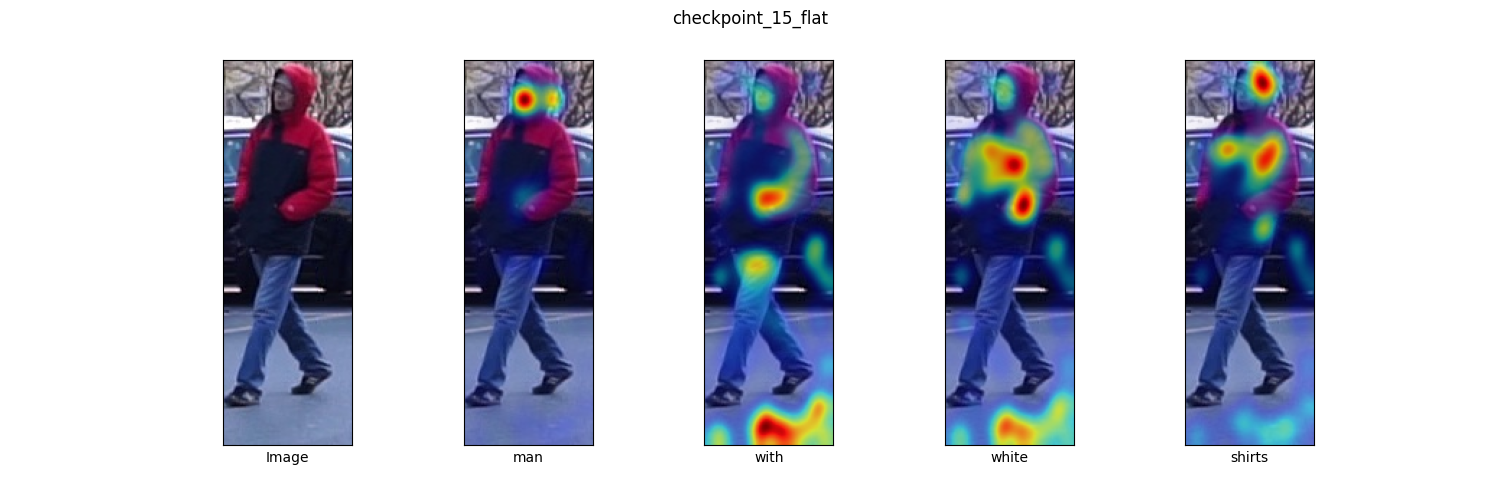
\includegraphics[width=\linewidth]{img/mlm2/mlm-checkpoint_15_flat.png}
  \caption{Visual grounding for masking ratio of 15 in \acrshort{mlm}}
  \label{fig:mlm_1}
\end{figure}

\begin{figure}[htbp]
  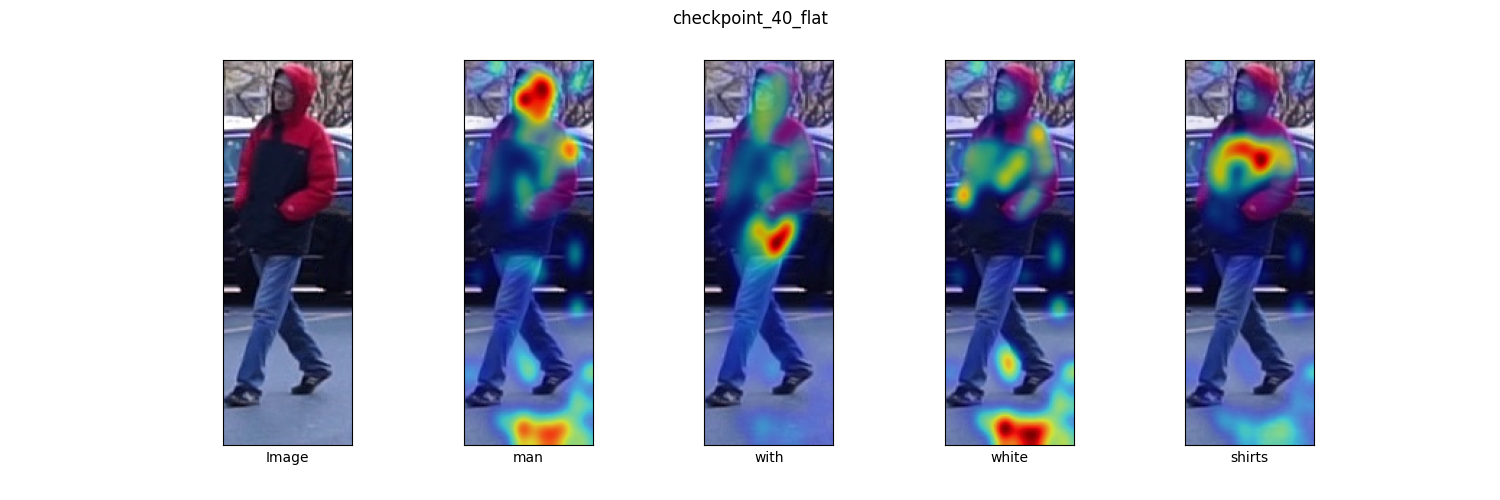
\includegraphics[width=\linewidth]{img/mlm2/mlm-checkpoint_40_flat.png}
  \caption{Visual grounding for masking ratio of 40 in \acrshort{mlm}}
  \label{fig:mlm_6}
\end{figure}

Similarly, in the case of the modified replacement token detection (m-rtd) approach, we did not observe any improvement in performance. The rationale behind this method was that by altering the masking rate, we could affect the number of words predicted during each training session. Specifically, we hypothesized that increasing the masking rate would lead to a greater volume of data being processed, which in turn would enhance the overall optimization and efficiency of the training process. This was based on the assumption that a higher masking rate would provide the model with more opportunities to learn from a larger set of masked tokens.

Despite this expectation, the experimental results did not align with our hypothesis. We found that even with a higher masking rate, there was almost no significant change in the performance of the model. Fig \ref{fig:mtrd_1} and \ref{fig:mtrd_6} shows that the attention region did not affect from the masking ratio. This outcome suggests that simply increasing the amount of masked data does not necessarily translate to better optimization or improved learning in this context. It highlights the complexity of the learning dynamics in such models and indicates that other factors might be at play that influence the effectiveness of the training process.


\begin{figure}[htbp]
  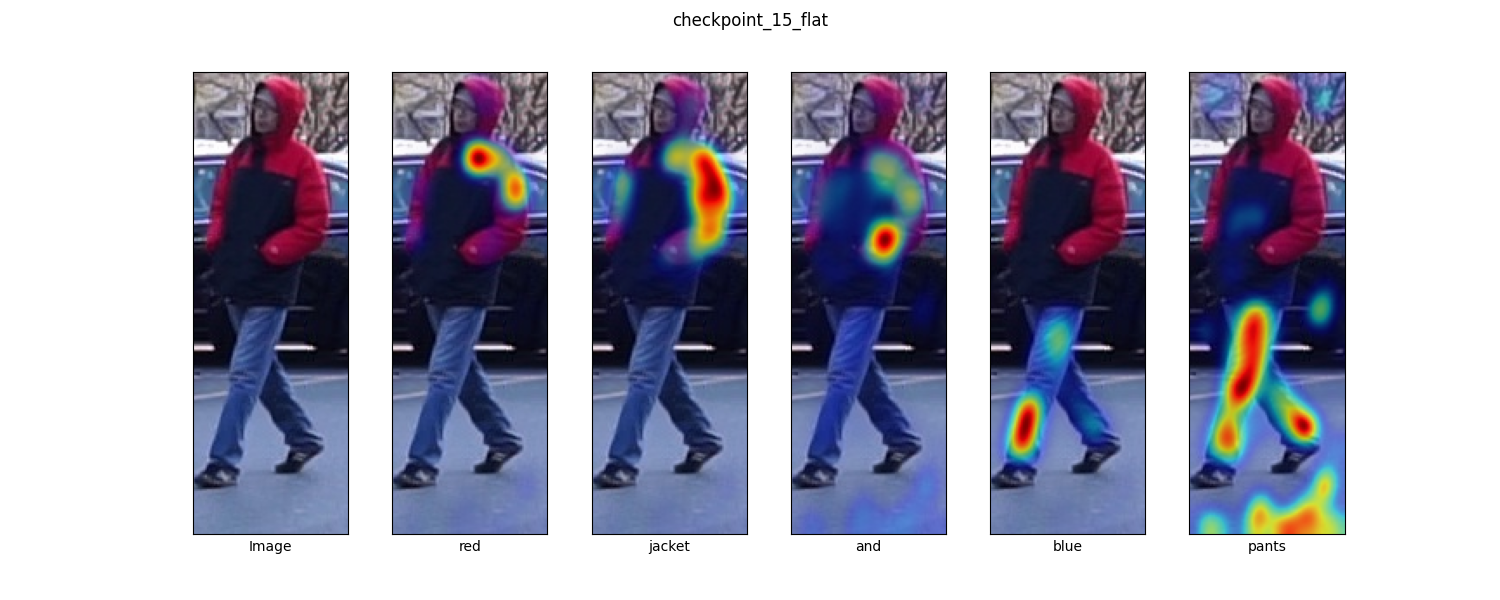
\includegraphics[width=\linewidth]{img/mrtd_masking_ratio/mrtd-checkpoint_15_flat.png}
  \caption{Visual grounding for masking rate of 15 in \acrshort{mrtd}}
  \label{fig:mtrd_1}
\end{figure}


\begin{figure}[htbp]
  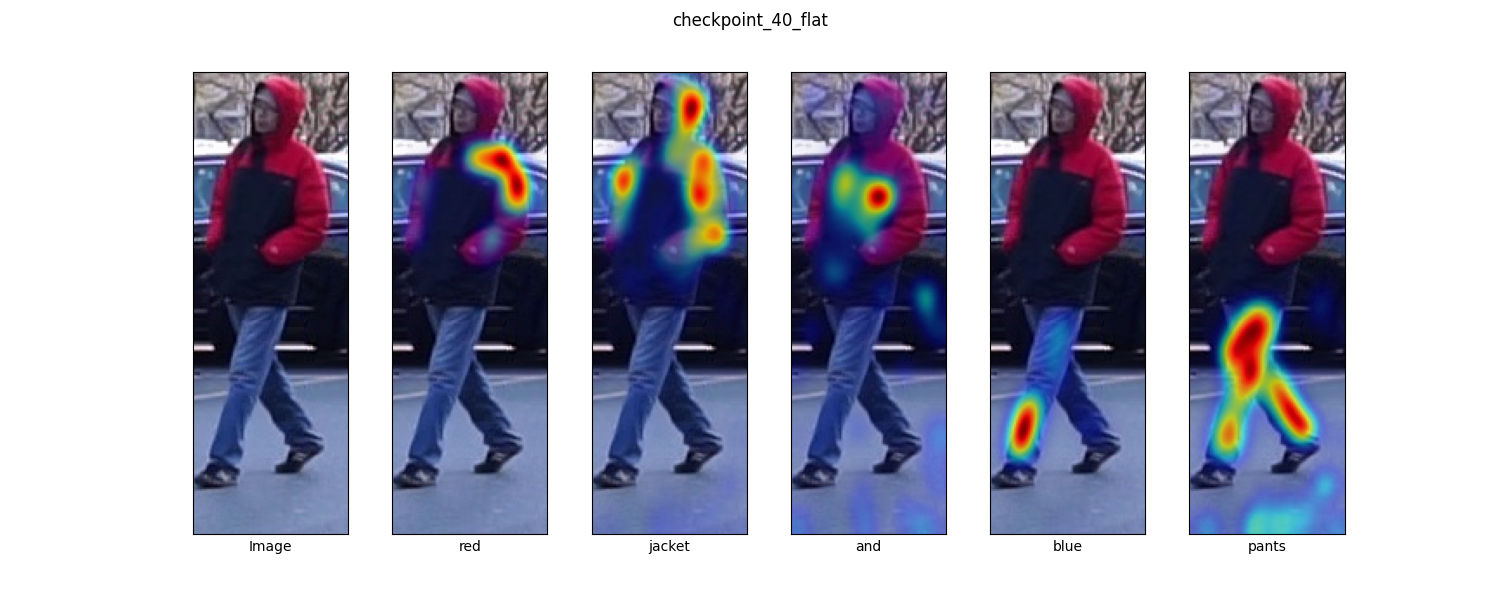
\includegraphics[width=\linewidth]{img/mrtd_masking_ratio/mrtd-checkpoint_40_flat.png}
  \caption{Visual grounding for masking rate of 40 in \acrshort{mrtd}}
  \label{fig:mtrd_6}
\end{figure}

Previous methodologies (\cite{devlin2018bert}) have highlighted the importance of pre-training steps in model development. During pre-training, the model learns to extract and integrate information from different modalities effectively. This stage significantly impacts the model's knowledge base, as it builds the foundational understanding necessary for downstream tasks. The analysis of pre-training steps in earlier work has shown that these steps are critical for the model's ability to generalize and perform well on diverse tasks.

% Fine-tuning is pivotal in achieving high performance on specific tasks because it tailors the model's capabilities to meet the requirements of the task at hand. However, the actual knowledge and understanding acquired during pre-training remain unchanged. Thus, the effectiveness of fine-tuning is highly dependent on the quality and relevance of the training data and tasks used during this stage. Selecting appropriate fine-tuning tasks that align with the target application is crucial for optimizing the model's performance.
Fine-tuning trains a model to produce an answer to a specific task, essentially adapting the model to a particular method or data set. This step is important to optimize the model's performance for a particular task, but does not fundamentally change the underlying knowledge of the model. The main function of fine tuning is to adapt the pre-trained model to the nuances of the target task so that the learned knowledge can be applied effectively. \ref{fig:rasa_comparison} is a result from \cite{Bai2023RaSaRA} with different settings from their model. Their work shows that the performance has improved with each additional feature. Therefore, from the results we have achieved, it is more effective to devise a method of extracting features suitable for the target task than to improve performance by changing the masking rate of the hyperparameters this time.

\begin{figure}[htbp]
  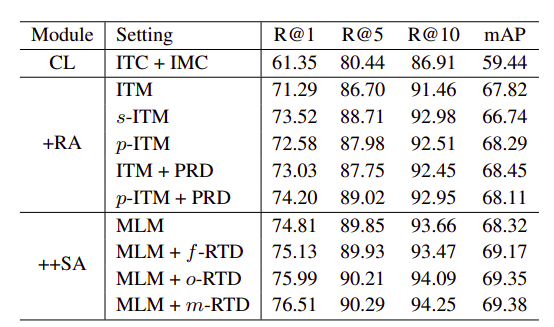
\includegraphics[width=\linewidth]{img/rasa_comparison.png}
  \caption{RaSa comparison with a different setting. ITM learns from all positive pairs without a probabilistic inputting. s-ITM learns from only strong positive pairs and discards all weak positive pairs. p-ITM uses a probabilistic inputting of strong and weak positive pairs. f-RTD adopts \cite{sanh2020distilbertdistilledversionbert} as a fixed generator to produce the replaced tokens. oRTD uses the online model as the generator, while m-RTD is based on the momentum model. Source from \cite{Bai2023RaSaRA}}
  \label{fig:rasa_comparison}
\end{figure}


% -- results line 
% talk about my work
%   check the numbers, use the visual grounding 
%   - training loss Graph
%   the results shows the loss prd, masking ratio, and loss mlm.
%   loss mlm correlates to the masking ratio, but prd decrease the same way for all 
%   - evaluation 
%   the r1~r10 does not change at all 

% -- discussion line
% discuss about the prediction 
% - my work didn't change at all 
% - for mlm, this method is major task for NLP and VLM models
% - previous method did an analysis in pre-training steps, which made significant difference because it's the part where the model actually learns how to achieve information from the modality
% - in fine-tuning, they're trained to generate the answers which corresponds to specific tasks
% - it's just fitting the model to specific method which does not effect that much to the actual model knowledge, that's why the fine-tuning part is more important to have better training task that really fits to the task you want the model to solve


